\documentclass[a4paper,11pt]{article}
\usepackage[utf8]{inputenc}
\usepackage[top=1.8cm,bottom=2.0cm,right=1.35cm,left=1.35cm]{geometry}
\usepackage{url}
\usepackage[natbibapa]{apacite}
\bibliographystyle{apacite}
\usepackage{graphicx}
\usepackage{amsmath}
\usepackage{amsfonts}
\usepackage{amssymb}
\usepackage[onehalfspacing]{setspace}
\usepackage{enumitem}
\usepackage{hyperref}
\usepackage{listings}
\usepackage{color}

\usepackage{lipsum}% this generates fictitious text for sample
%opening
\title{Twitter Dataset Analysis\\ Group 17}
\author{
    \begin{tabular}{lll}
    \textbf{Name} & \textbf{Student Number (SN)} & \textbf{Contribution} \\
    Karan Goel & 7836685 & 14.28\% \\
    Alvin Jose & 8066358 & 14.28\% \\
    Ashutosh Bhosale & 7795786 & 14.28\% \\
    Banin Sensha Shreshta & 8447196 & 14.28\% \\
    Gaurav Adarsh Santosh & 7032663 & 14.28\% \\
    Lino Thankachan & 7926017 & 14.28\% \\
    Rishab Manokaran & 7863974 & 14.28\% \\
    \end{tabular}
}


\date{CSCI946 Big Data Analytics Assignment 2\\
September 20, 2024}

\begin{document}
\maketitle
\newpage
\section{Introduction}

In this assignment, the primary objective is to detect misinformation on social networks by identifying profiles that are incorrectly classified as human or non-human. The focus of the analysis will be on the Twitter user dataset, where we aim to explore methods to distinguish between genuine and artificially generated accounts. To achieve this, we will follow a structured approach outlined in Tasks 1-4.

Task 1 involves designing a comprehensive big data analytics project, adhering to the principles of the Big Data Analytics Lifecycle.

In Task 2, the dataset will be processed by taking into account the various data types and properties. Core models and algorithms will be applied, including regression, association rules, clustering, classification, and text processing methods.

Task 3 focuses on visualizing the dataset and utilizing visual representations to evaluate the analysis results. This step will provide valuable insights into the data and help validate the findings.

Finally, Task 4 entails a detailed study of various profile factors, such as text, color, and tweet content. Based on this analysis, recommendations will be made to adjust the classification of human and non-human profiles.

\section{Task 1: Data Analysis Design}

\subsection{Learn Business Domain}
\textbf{Objective}: The aim of assignment this is to identify profiles on social networks that are mistakenly recorded as human or non-human profiles (e.g., bots).\\
\textbf{Specific Task}: You need to identify if the user’s gender is either human (male, female) or non-human(brand) based on their Twitter profile data and associated tweets.\\
\textbf{Dataset}: The dataset for this classification task can be accessed via Kaggle at the \href{https://www.kaggle.com/datasets/crowdflower/twitter-user-gender-classification}{Twitter User Gender Classification dataset}.

\subsection{Define Resources \& Goals}
\textbf{Data Source}: Twitter user profiles including tweets, descriptions, link color, sidebar color, and other metadata.\\
\textbf{Primary Task}: Classify gender into two categories: human or non-human.\\
\textbf{Key Questions}:
\begin{itemize}
    \item How well do the words in tweets and profiles predict the user as human or non-human?
    \item What are the specific words that strongly predict human or non-human?
    \item How well do other factors (like link color, tweet count, retweet count, favourite number) predict user as human or non-human?
\end{itemize}

\subsection{Frame the Problem \& Develop Initial Hypotheses}
\textbf{Problem Type}: This is a supervised learning problem where the task is to predict a categorical variable (gender: male, female, or brand).\\
\textbf{Hypotheses}:
\begin{itemize}
    \item \textbf{Null Hypothesis (H0)}: Words in tweets and profiles do not have a significant effect on predicting user gender (i.e., the predictive power is random or weak).
    \item \textbf{Alternative Hypothesis (H1)}: Words in tweets and profiles have a significant effect on predicting user gender (i.e., they provide strong predictive power).
    \item \textbf{Additional Hypotheses}:
    \begin{itemize}
        \item \textbf{H0}: Stylistic factors (link color, sidebar color) are not good predictors of gender.
        \item \textbf{H1}: Stylistic factors can strongly predict gender.
    \end{itemize}
\end{itemize}

\subsection{Data Preparation}
\textbf{Preprocessing Steps}:
\begin{itemize}
    \item \textbf{Stemming \& Lemmatization}: To reduce words to their base or root forms.
    \item \textbf{Lowercasing}: To eliminate discrepancies between uppercase and lowercase letters.
    \item \textbf{Tokenization}: Split text into individual words or tokens.
    \item \textbf{Embedding}: Use word embeddings (e.g., Word2Vec, GloVe, or TF-IDF) to represent text data numerically.
    \item \textbf{Bag of Words}: A simple and effective method for text representation.
    \item \textbf{Word2Vec}: A simple model to generate world embeddings.
\end{itemize}

\subsection{Visualize Data}
\textbf{Visualization Techniques}:
\begin{itemize}
    \item \textbf{Word Cloud}: To display frequent words by gender category (male/female/brand).
    \item \textbf{Word Distance/Similarity}: Use techniques like cosine similarity to understand which words or phrases are closer to each gender category.
\end{itemize}

\subsection{Model Building}
\textbf{Classification Models}:
\begin{itemize}
    \item \textbf{K-Nearest Neighbors (KNN)}, \textbf{Support Vector Machines (SVM)}, \textbf{Decision Trees}, \textbf{Random Forest}.
\end{itemize}
\textbf{Clustering Models}:
\begin{itemize}
    \item \textbf{K-Means}, \textbf{DBSCAN}, \textbf{Self-Organizing Maps (SOM)}.
\end{itemize}
\textbf{Regression Models}:
\begin{itemize}
    \item \textbf{Linear Regression}, \textbf{Logistic Regression}.
\end{itemize}
\textbf{Neural Networks}:
\begin{itemize}
    \item Build deep learning models to classify gender using \textbf{Neural Networks}.
\end{itemize}

\subsection{Training and Testing}
\textbf{Cross-Validation}: Use \textbf{k-fold cross-validation} to prevent overfitting and assess model generalization.\\
\textbf{Grid Search}: Optimize hyperparameters by performing grid search to select the best model configuration.

\subsection{Deliverables}
\textbf{Evaluation Metrics}:
\begin{itemize}
    \item \textbf{Confusion Matrix}: To visualize the performance of each classification model.
    \item \textbf{Accuracy}: The percentage of correctly classified instances.
    \item \textbf{Precision}: The proportion of true positives out of all positive predictions.
    \item \textbf{Recall}: The proportion of true positives out of all actual positives.
    \item \textbf{Loss Curves}: For neural networks, to visualize the training process and detect overfitting or underfitting.
\end{itemize}


\section{Task 2: Data Processing \& Model Application}

The dataset was loaded using the \texttt{load\_data} method from the \texttt{Task1} class, which reads a CSV file containing Twitter user data. After loading, the data was preprocessed to make it suitable for the classification task.

\subsection{Data Filtering}
\begin{itemize}
    \item Rows with a \texttt{gender:confidence} score greater than 0.9 were selected to ensure data quality.
    \item The \texttt{gender} labels were restricted to three categories: \texttt{male}, \texttt{female}, and \texttt{brand}.
    \item The \texttt{gender} column was relabeled: \texttt{male} and \texttt{female} were grouped into a \texttt{human} class, while \texttt{brand} was grouped into the \texttt{non-human} class.
\end{itemize}

\subsection{Handling Missing Values}
Missing values were filled with empty strings (\texttt{''}) to avoid issues during text processing and model training.

\subsection{Feature Selection}
The key features selected for the classification task were \texttt{gender}, \texttt{fav\_number}, \texttt{retweet\_count}, \texttt{tweet\_count}, and \texttt{text}.

\subsection{Feature Scaling and Label Encoding}
Two important steps were applied to further process the numerical and categorical data:

\subsubsection{Scaling Features}
We used \texttt{StandardScaler} to normalize numerical features such as \texttt{fav\_number}, \texttt{retweet\_count}, and \texttt{tweet\_count}. This step ensures that all features are on a similar scale, improving the performance of machine learning algorithms.

\subsubsection{Label Encoding}
The \texttt{gender} column was encoded using \texttt{LabelEncoder} to convert the \texttt{human} and \texttt{non-human} categories into numerical labels.

\subsection{Exploratory Data Analysis}
To better understand the relationships between features, we performed the following analyses:

\subsubsection{Correlation Matrix}
We computed the correlation matrix for the numerical features to observe the strength of linear relationships between variables. P-values were calculated for each pair of features to identify significant correlations. A heatmap was generated to visualize only significant correlations (with p-values less than 0.05). Figure \ref{fig:corr}

\subsubsection{Pairplot}
A scatterplot matrix (pairplot) was created to visualize relationships between the numerical features. This helped in detecting patterns and potential outliers in the dataset. Figure \ref{fig:p_plot}

\subsection{Text Processing}
Since the core of this classification task involves analyzing text data (tweets), we employed several text preprocessing techniques:

\subsubsection{Denoising}
The text was cleaned by removing unwanted characters such as URLs, HTML tags, punctuation, hashtags, and special characters using various utility methods such as \texttt{remove\_html}, \texttt{remove\_url}, and \texttt{remove\_punctuation}.

\subsubsection{Standardization}
All text was converted to lowercase using the \texttt{standardize\_text} method to avoid case-sensitive discrepancies.

\subsubsection{Lemmatization}
The \texttt{WordNetLemmatizer} was used to reduce words to their base forms (lemmas), making the text more uniform for the model while preserving meaning.

\subsubsection{Stopword Removal}
Common stopwords (e.g., ``and'', ``the'', ``is'') and irrelevant words like ``RT'', ``like'', and ``follow'' were removed to focus on meaningful words.

\subsubsection{Word Cloud Visualization}
A word cloud was generated to visualize the most frequent words across all tweets, providing insight into the dominant terms associated with the gender categories. Figure \ref{fig:wc}

\subsection{Feature Extraction}
To convert the processed text data into a numerical format suitable for machine learning models, we employed two feature extraction techniques:

\subsubsection{Bag of Words (BoW)}
The text data was vectorized using \texttt{CountVectorizer}, transforming the text into a sparse matrix of token counts. This simple and effective method allowed us to represent the frequency of words in each tweet. The resulting dense array was stored in the dataset as the \texttt{bow\_feature}. This Bow can be seen in added in this Figure \ref{fig:df}.

\subsubsection{Word2Vec Embeddings}
Word2Vec embeddings were computed using the \texttt{Word2Vec} model from the Gensim library. This method captured semantic information by learning distributed vector representations of words. The average embedding for each tweet was calculated and stored as \texttt{word2vec\_embeddings} in the dataset.

\section{Task 3: Visualization}

\begin{figure}[h!]
    \centering
    \begin{minipage}{0.45\textwidth}
        \centering
        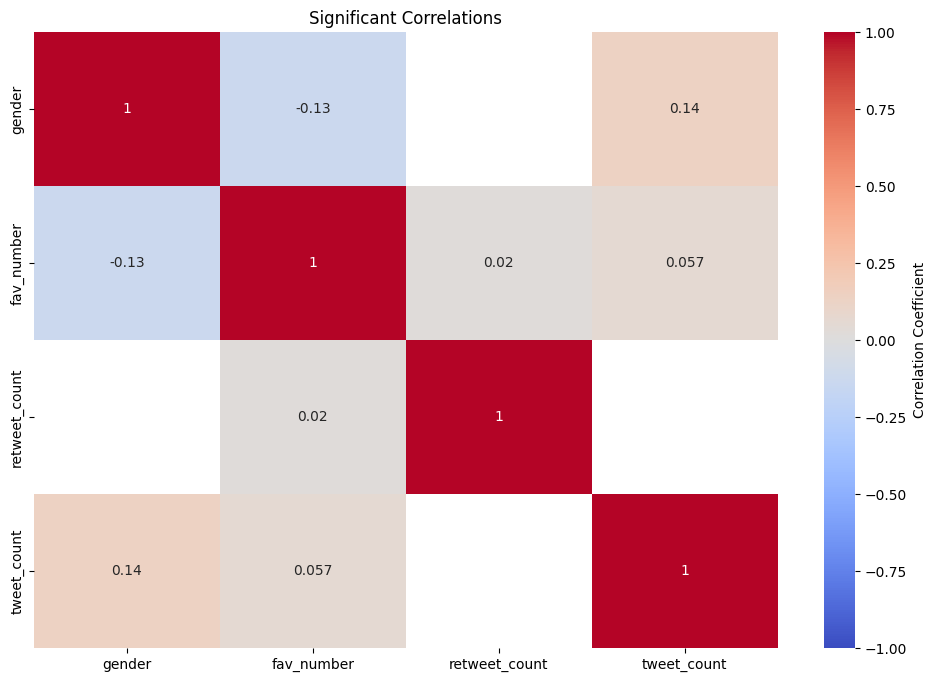
\includegraphics[width=\textwidth]{corr_a2.png}
        \caption{Correlation Matrix}
        \label{fig:corr}
    \end{minipage}
    \hfill
    \begin{minipage}{0.45\textwidth}
        \centering
        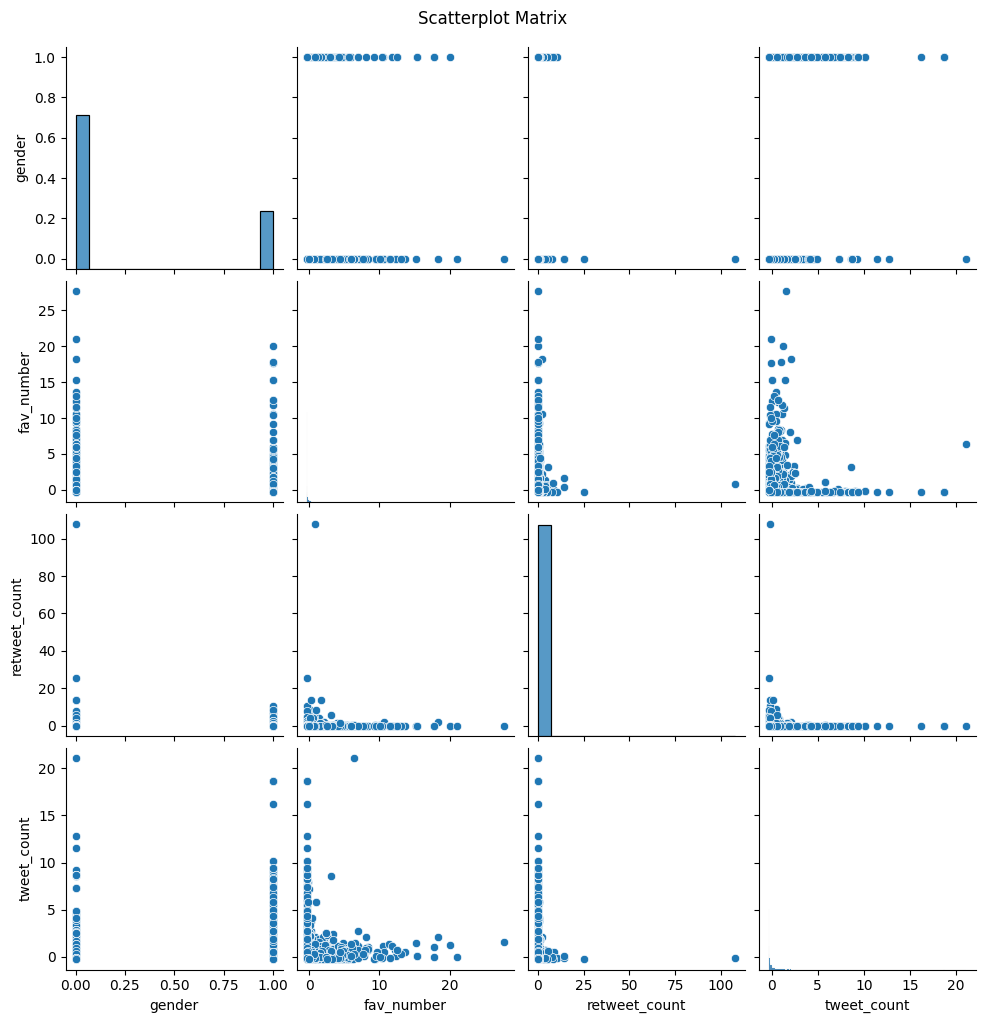
\includegraphics[width=\textwidth]{pair_plot_a2.png}
        \caption{Pair Plot}
        \label{fig:p_plot}
    \end{minipage}
\end{figure}

\begin{figure}[h!]
    \centering
    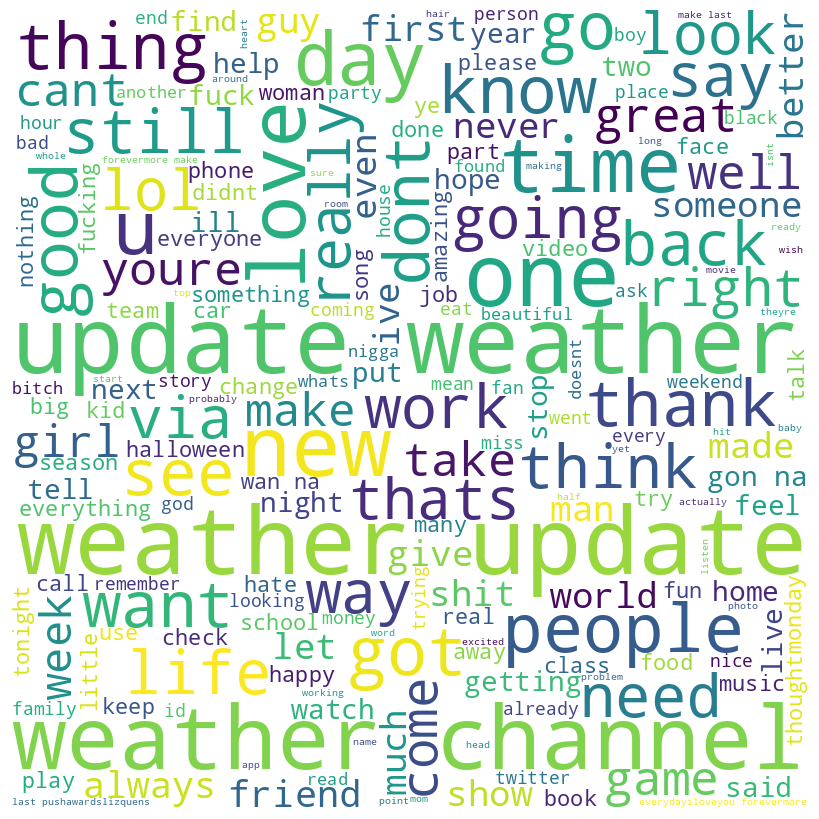
\includegraphics[width=0.5\textwidth]{word_cloud_a2.png}
    \caption{Word Cloud}
    \label{fig:wc}
\end{figure}

\begin{figure}[h!]
    \centering
    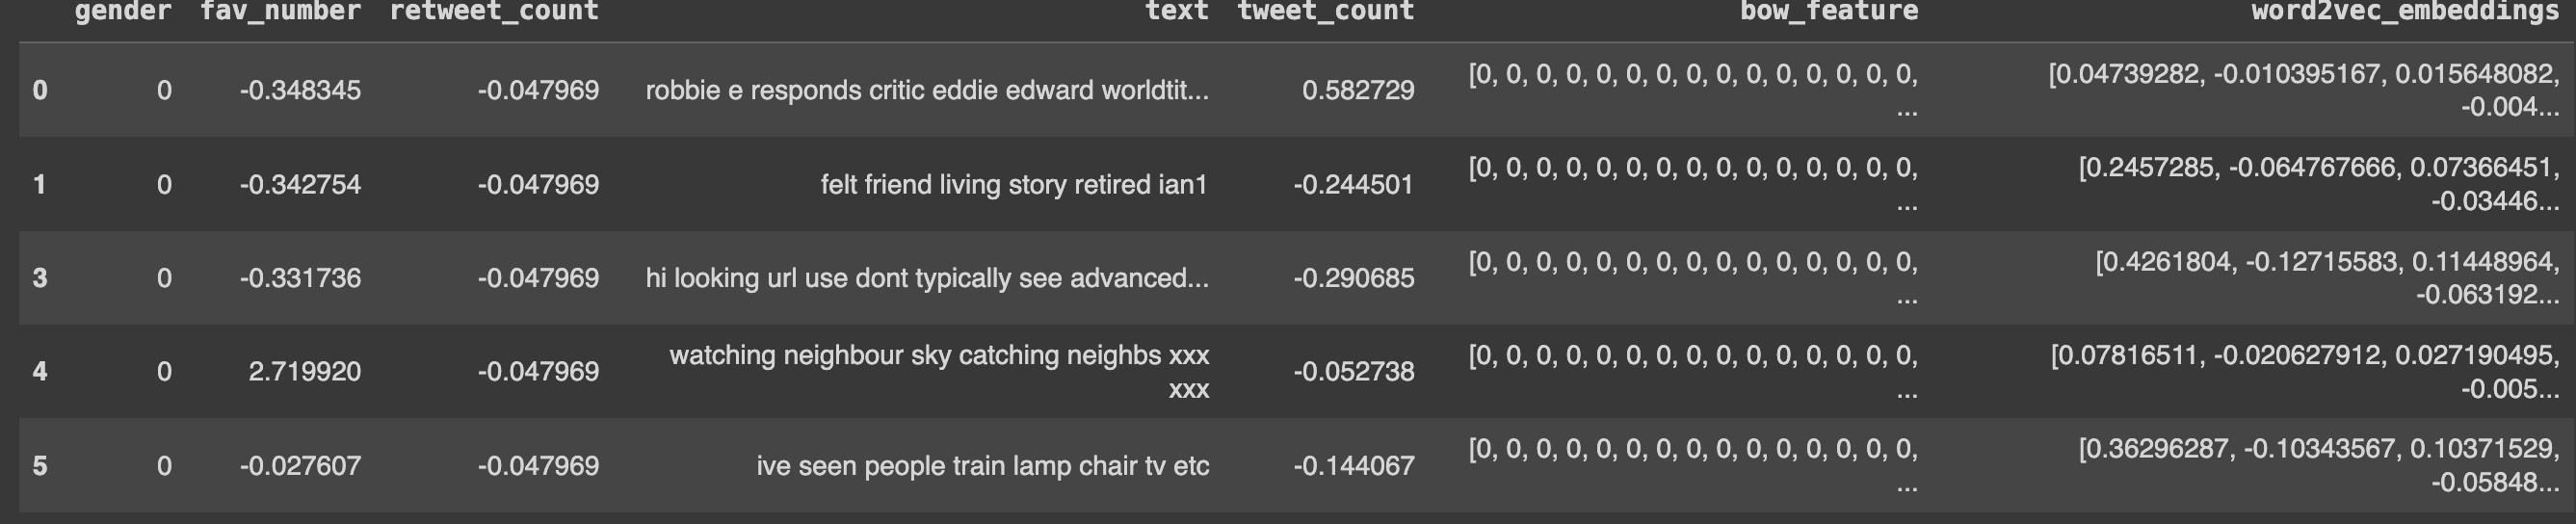
\includegraphics[width=0.5\textwidth]{df.png}
    \caption{Data Frame}
    \label{fig:df}
\end{figure}


\newpage
\bibliography{bibliography_data}
\nocite{*}
\end{document}
